\subsubsection{Requirements}

For a given chess position and a played move, the commentator should create comments on different categories. Those categories are the \textit{description of the current move}, the \textit{description of the move quality}, the \textit{comparison of moves}, the \textit{description of the move planning} and \textit{contextual game information}.\footnote{Cf. Jhamtani et al. 2018 p. 3}$^{,}$\footnote{Cf. Zang et al. 2019, pp. 3-4}

\begin{figure}[h]
\centering
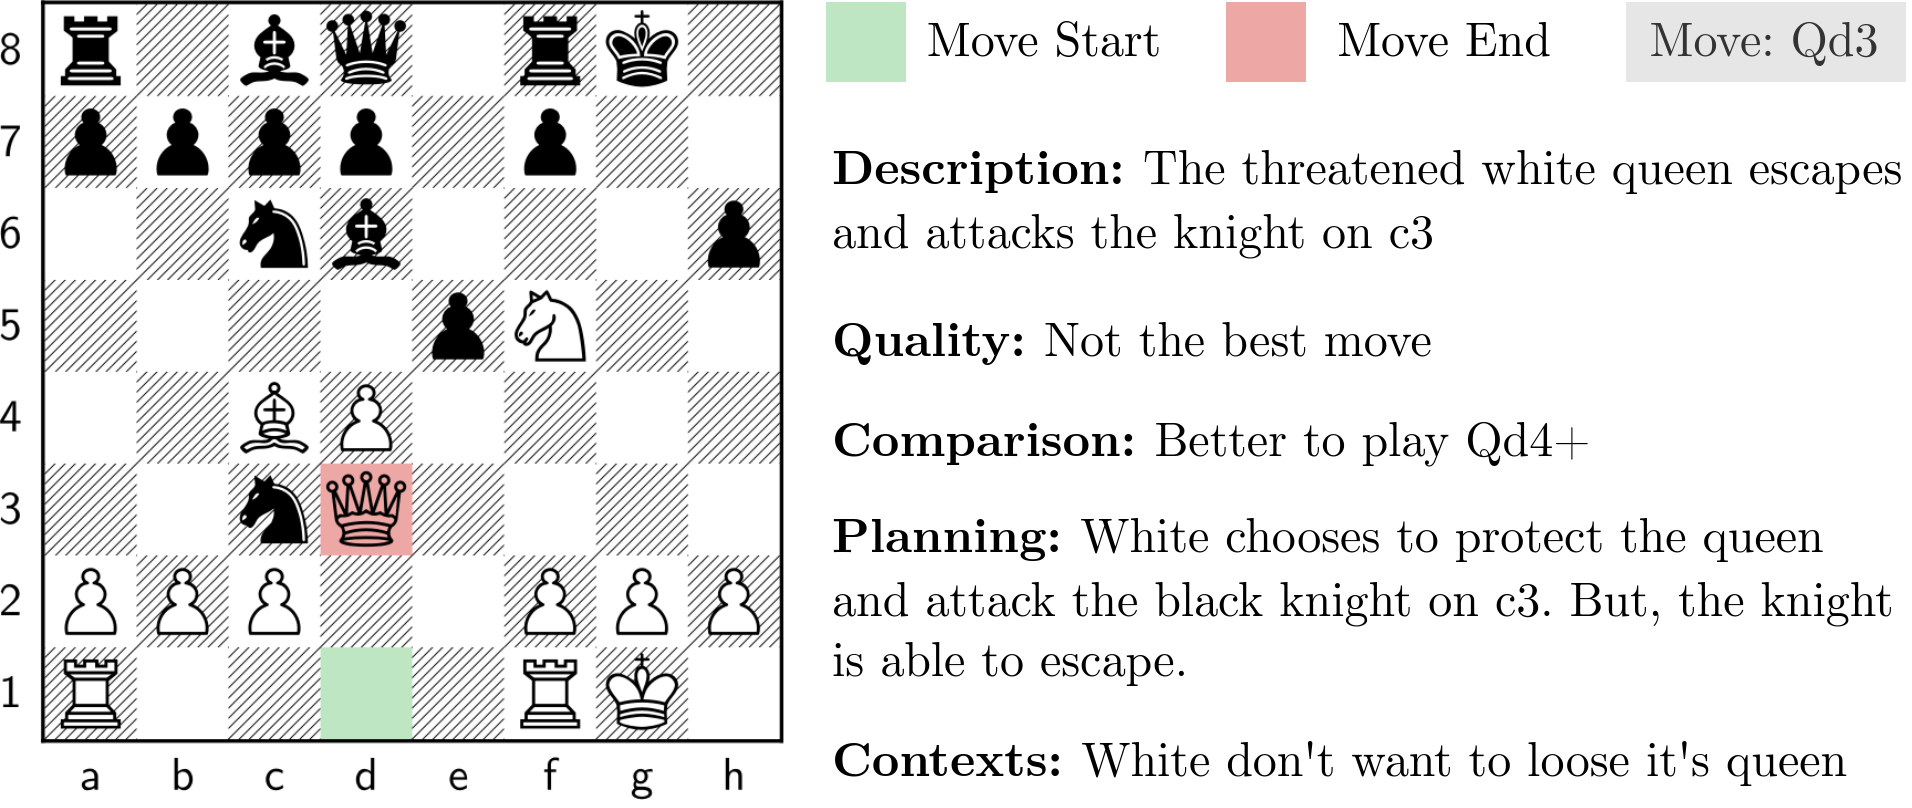
\includegraphics[width=0.7\textwidth]{graphics/commentator_example/commentator.png}
\caption{Chess Commentary Example (Note: Figure based on \cite{zang-etal-2019-automated} Figure 1)}
\end{figure}

These requirements can be divided according to the number of moves and positions considered for the generation. There are categories that require only one position and the played move (description and quality), and cateogries that require multiple positions and moves (comparison, planning and context) so that the description is accurate.

Since the procedure for creating comments varies from category to category, it is practically impossible to do this with a single commentator, as simplified described above. Therefore, in the following it will be spoken of five individual ones, each for one of the categories. In addition, instead of categories, it is now spoken of generation models, since these are used to generate comments.

% These requirements come with two challenges that can have a strong impact on the quality of the generated description: (1) the features on the basis of which the comments for the aspects are generated, (2) the number of moves and the resulting position considered. To overcome the first challenge \cite{jhamtani-etal-2018-learning} used "discrete information (threats, game evaluation scores, etc.)"\footnote{Zang et al. 2019 p. 4}. How \cite{zang-etal-2019-automated} show, those features information did not provide the best results. Therefore, they have used features provided directly by the internal chess engine. These are the \textit{state of the board before the move}, \textit{start square of the move}, \textit{end square of the move}, \textit{piece on the start square}, \textit{piece on the end square}, \textit{promotion state} and  \textit{checking state}. The pieces on the starting square and on the ending square can be different, since the pawns can be replaced by another piece when they reach the opponent's last rank.\footnote{See \cite{fide-2018-loc} p. 6} In this case the promotion state would be set to true. The advantage of using these features is that they can be easily read from the information provided by the chess engine described in the previous section. The second challenge can be overcome by distinguishing between requirements that need only one move (description and quality) and requirements that need multiple moves (comparision, planning and context) so that the description is accurate.

% With these challenges overcomed the next steps are

% Once these problems are solved, for each requirement, the information needed to fulfill a requirement must be put into a form that can be used as input, certain features can be easily identified, and the text can be generated based on these identifications.

% In order to generate comments on these requirements, it is necessary to define certain features on the basis of which this is done. \cite{jhamtani-etal-2018-learning} uses features such as, \gls{threats} and position value, but as \cite{zang-etal-2019-automated} show, this information does not consider the following positions well enough, which affects the quality of comments. To solve this problem the requirements were divided into two categories: (1) requirements which need exactly one move to be describe, (2) requirements which need a number of moves to be describe. The second category is only an extension of the first, so the two categories differ in detail only in how many positions and moves they consider; the features included remain the same.

% A method which has shown significant success in the field of natural language processing are Recurrent Neural Networks (RNN).

% The process of generating the text commentary can be summarized into two upper parts, namely encoding and decoding. Encoding describes the extraction and formatting of certain features to make them easier to process, while decoding describes the translation of the encoded features into a text format.